\documentclass[ignorenonframetext,]{beamer}
\setbeamertemplate{caption}[numbered]
\setbeamertemplate{caption label separator}{: }
\setbeamercolor{caption name}{fg=normal text.fg}
\beamertemplatenavigationsymbolsempty
\usepackage{lmodern}
\usepackage{amssymb,amsmath}
\usepackage{ifxetex,ifluatex}
\usepackage{fixltx2e} % provides \textsubscript
\ifnum 0\ifxetex 1\fi\ifluatex 1\fi=0 % if pdftex
  \usepackage[T1]{fontenc}
  \usepackage[utf8]{inputenc}
\else % if luatex or xelatex
  \ifxetex
    \usepackage{mathspec}
  \else
    \usepackage{fontspec}
  \fi
  \defaultfontfeatures{Ligatures=TeX,Scale=MatchLowercase}
\fi
\usecolortheme{seahorse}
\usefonttheme{structurebold}
% use upquote if available, for straight quotes in verbatim environments
\IfFileExists{upquote.sty}{\usepackage{upquote}}{}
% use microtype if available
\IfFileExists{microtype.sty}{%
\usepackage{microtype}
\UseMicrotypeSet[protrusion]{basicmath} % disable protrusion for tt fonts
}{}
\newif\ifbibliography
\hypersetup{
            pdftitle={Usando y Enseñando R para Investigación Reproducible},
            pdfborder={0 0 0},
            breaklinks=true}
\urlstyle{same}  % don't use monospace font for urls
\usepackage{graphicx,grffile}
\makeatletter
\def\maxwidth{\ifdim\Gin@nat@width>\linewidth\linewidth\else\Gin@nat@width\fi}
\def\maxheight{\ifdim\Gin@nat@height>\textheight0.8\textheight\else\Gin@nat@height\fi}
\makeatother
% Scale images if necessary, so that they will not overflow the page
% margins by default, and it is still possible to overwrite the defaults
% using explicit options in \includegraphics[width, height, ...]{}
\setkeys{Gin}{width=\maxwidth,height=\maxheight,keepaspectratio}

% Prevent slide breaks in the middle of a paragraph:
\widowpenalties 1 10000
\raggedbottom

\AtBeginPart{
  \let\insertpartnumber\relax
  \let\partname\relax
  \frame{\partpage}
}
\AtBeginSection{
  \ifbibliography
  \else
    \let\insertsectionnumber\relax
    \let\sectionname\relax
    \frame{\sectionpage}
  \fi
}
\AtBeginSubsection{
  \let\insertsubsectionnumber\relax
  \let\subsectionname\relax
  \frame{\subsectionpage}
}

\setlength{\parindent}{0pt}
\setlength{\parskip}{6pt plus 2pt minus 1pt}
\setlength{\emergencystretch}{3em}  % prevent overfull lines
\providecommand{\tightlist}{%
  \setlength{\itemsep}{0pt}\setlength{\parskip}{0pt}}
\setcounter{secnumdepth}{0}
\setbeamertemplate{navigation symbols}{}
\setbeamertemplate{footline}[page number]

\title{Usando y Enseñando R para Investigación Reproducible}
\author{Rayna M. Harris\\
Twitter: @raynamharris\\
página web: \url{https://raynamharris.github.io}\\}
\date{27 Marzo 2018\\
R-Ladies Buenos Aires}

\begin{document}
\frame{\titlepage}

\begin{frame}{¿Quién soy?}


\includegraphics{../figures/10_talk/twitter.png} \footnote<.->{\url{https://twitter.com/raynamharris}}

\end{frame}

\begin{frame}{Soy voluntaria de Sofware Carpentry}


\includegraphics{../figures/10_talk/swc1.png}

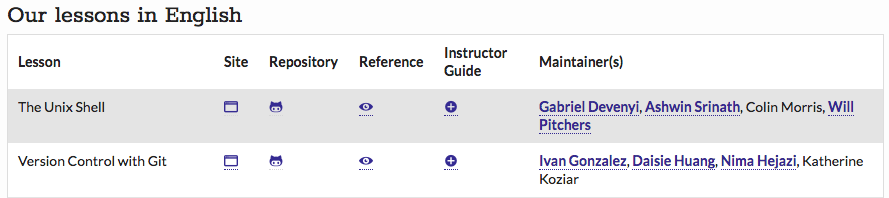
\includegraphics{../figures/10_talk/swc2.png}

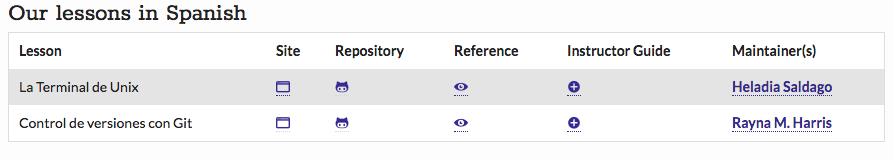
\includegraphics{../figures/10_talk/swc3.png} \footnote<.->{\textbf{cowplot}
  \url{https://cran.r-project.org/web/packages/cowplot/index.html}}

\end{frame}

\begin{frame}{Mis mejores 8 deseos con consejos}

\begin{itemize}[<+->]
\tightlist
\item
  Pero antes de comenzar
\item
  Recuerda que vos podés hacer lo que quieras
\item
  Recuerda que nadie es re buena al principio
\item
  Yo creo que la mejor manera de aprender es a ensenñar
\item
  Yo creo que todos aprenden más cuando la ciencia y la educación están
  abiertas
\end{itemize}

\end{frame}

\begin{frame}{Deseo 1: Desarrolla tu propia paleta de colores}

Colorbrewer\footnote<.->{\url{http://colorbrewer2.org/}} te ayuda a
elegir colores amigables para daltónicos

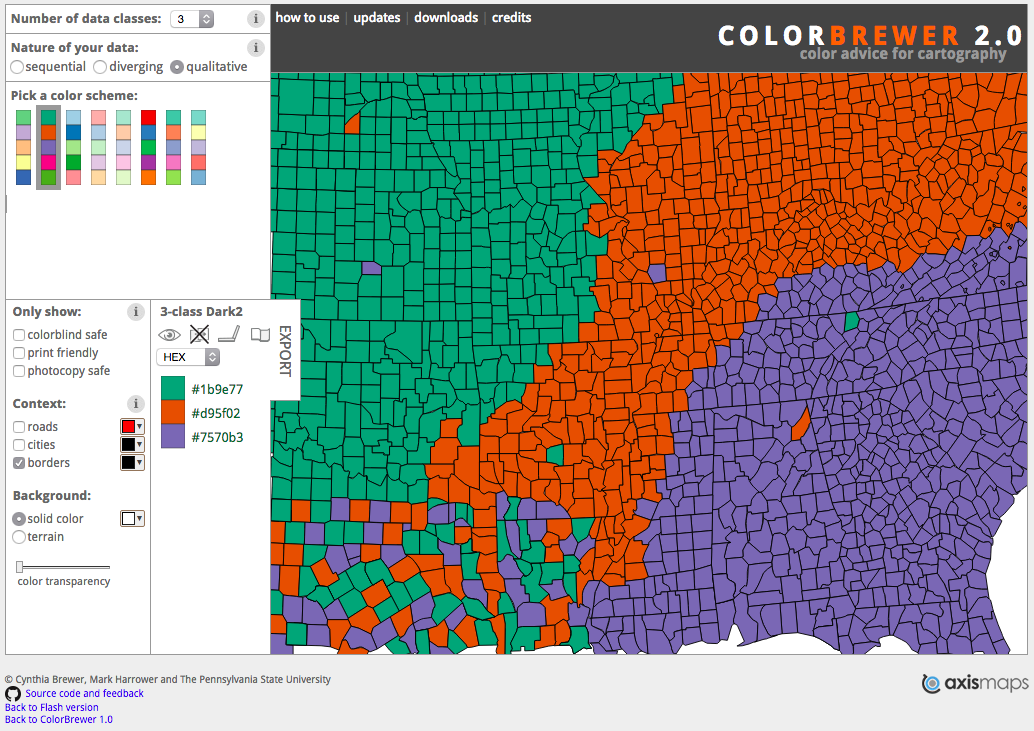
\includegraphics[width=0.75000\textwidth]{../figures/10_talk/colorbrewer.png}

\end{frame}

\begin{frame}[fragile]{Ejemplos de paletas de colores}

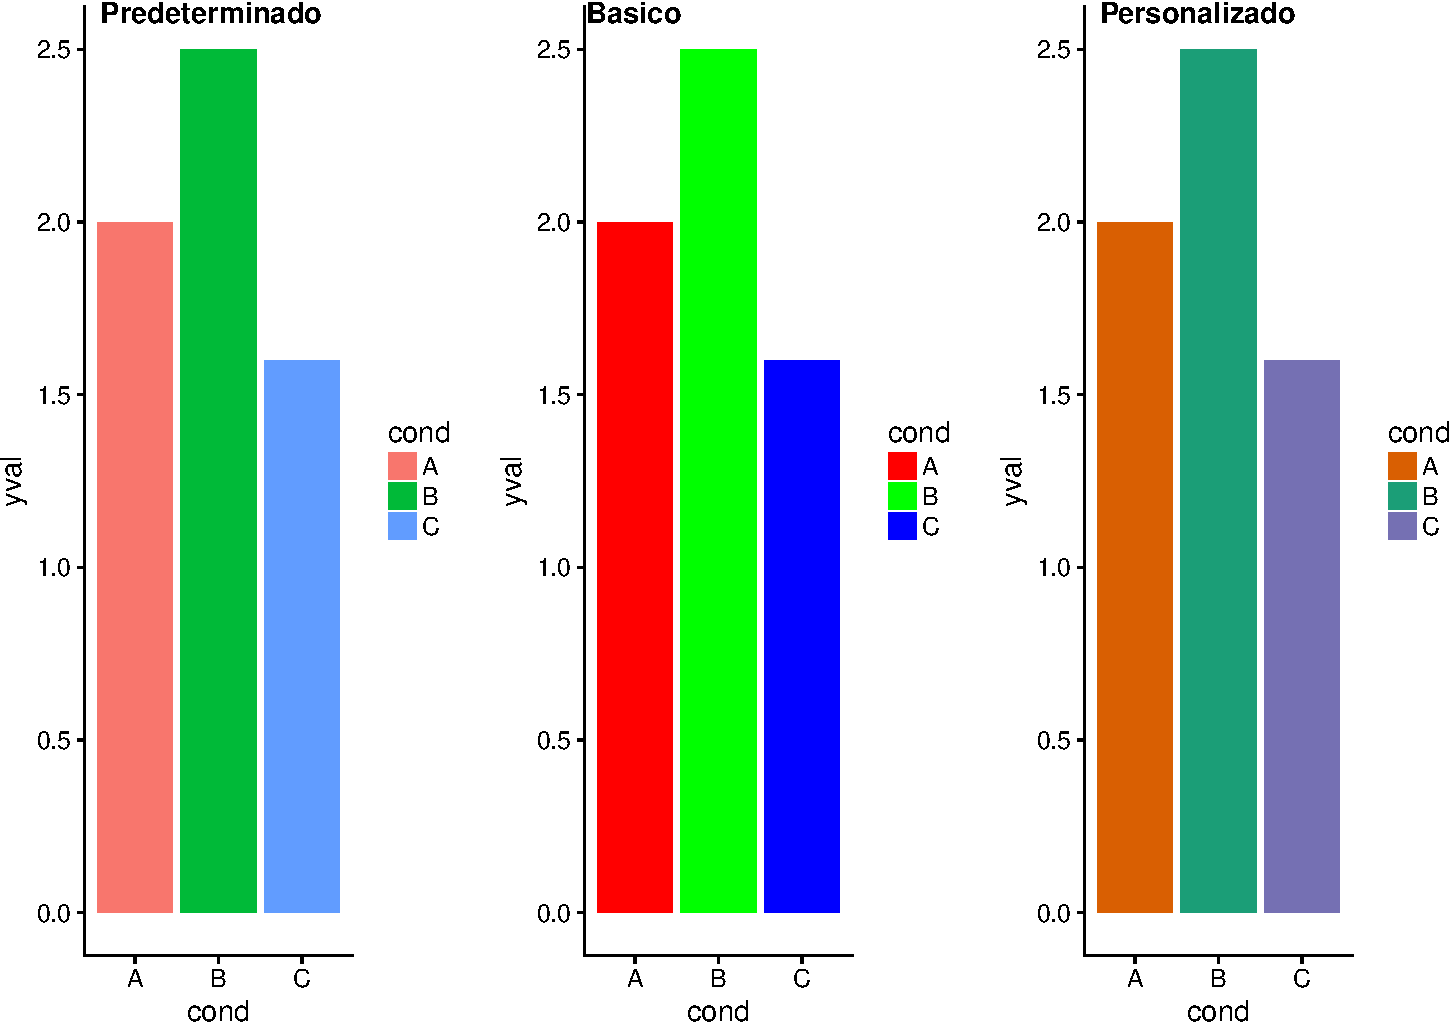
\includegraphics[width=225px]{../figures/10_talk/ejemplo-1}

\begin{itemize}
\tightlist
\item
  Basico:
  \texttt{+\ scale\_fill\_manual(values=c("red",\ "green",\ "blue"))}
\item
  Personalizado:
  \texttt{+\ scale\_fill\_manual(values=c("\#d95f02",\ "\#1b9e77",\ "\#7570b3"))}
\end{itemize}

\end{frame}

\begin{frame}{Convertir HEX a RGB si fuera necesario}

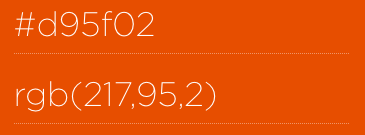
\includegraphics[width=0.50000\textwidth]{../figures/10_talk/orange.png}

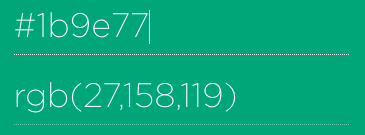
\includegraphics[width=0.50000\textwidth]{../figures/10_talk/teal.png}

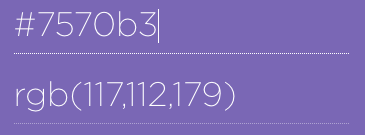
\includegraphics[width=0.50000\textwidth]{../figures/10_talk/purple.png}
\footnote<.->{\url{https://www.webpagefx.com/web-design/hex-to-rgb/}}

\end{frame}

\begin{frame}{Confirmá que tu paleta es amigable con los daltónicos}

colorblindr\footnote<.->{\url{https://github.com/clauswilke/colorblindr}}
simula deficiencias de visión del color

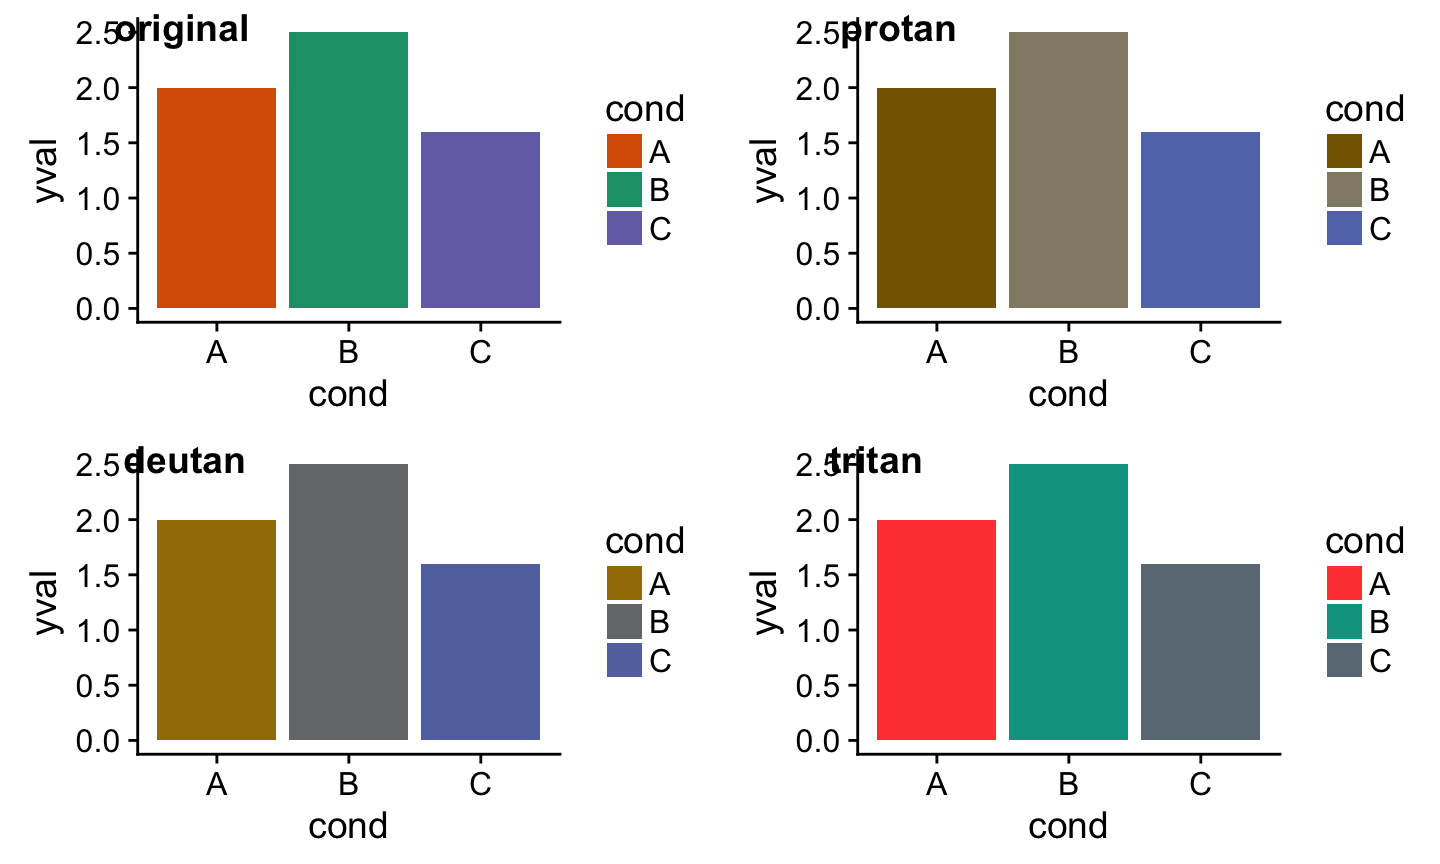
\includegraphics[width=225px]{../figures/10_talk/colorblindgrid-1}

\end{frame}

\begin{frame}{Deseo 2: Usa leyendas gráficas}

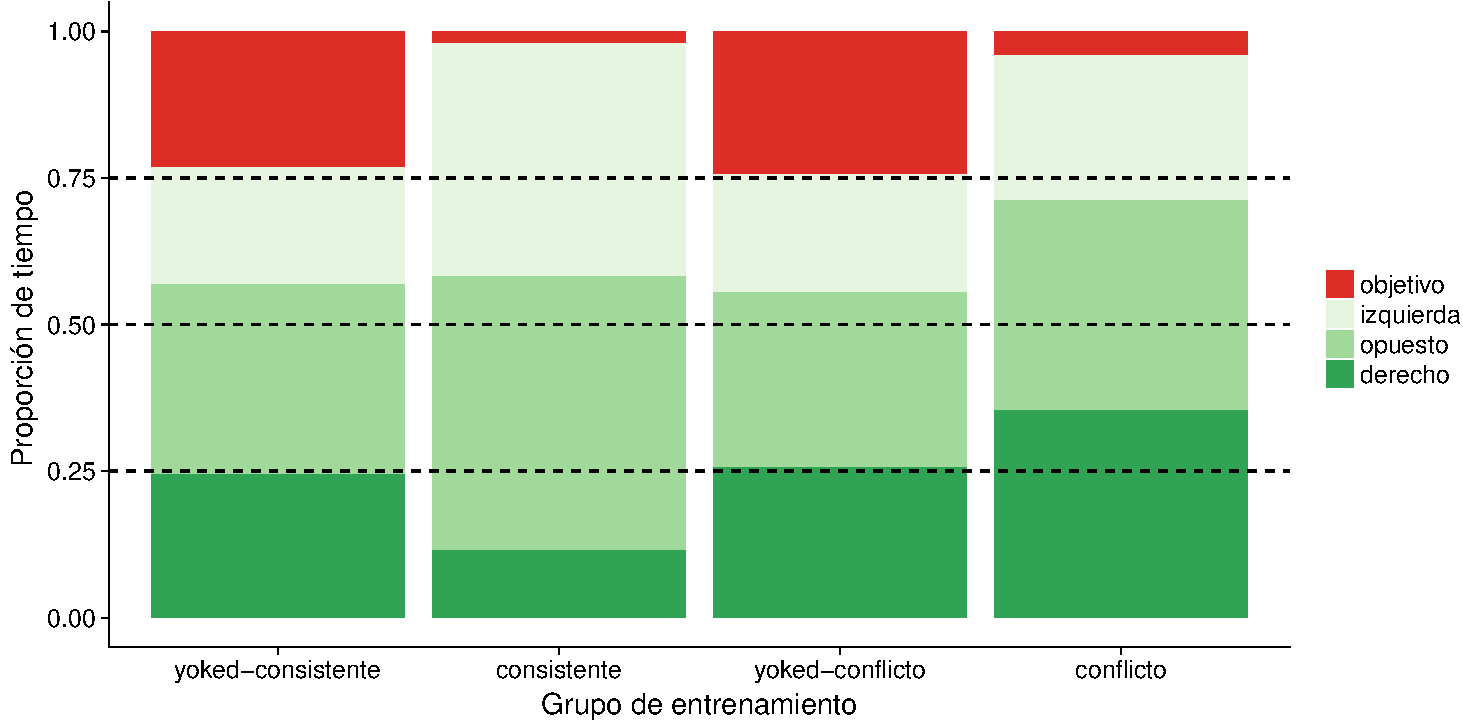
\includegraphics{../figures/10_talk/timespent-1.pdf}

\begin{itemize}[<+->]
\tightlist
\item
  ¿Qué significa ``objetivo'', ``izquierda'', ``opuesto'' y ``derecho''?
\item
  ¿Por qué el rosa ``objetivo''?
\item
  ¿Por qué hay líneas discontinuas?
\end{itemize}

\end{frame}

\begin{frame}{Deseo 2: Usa leyendas gráficas}

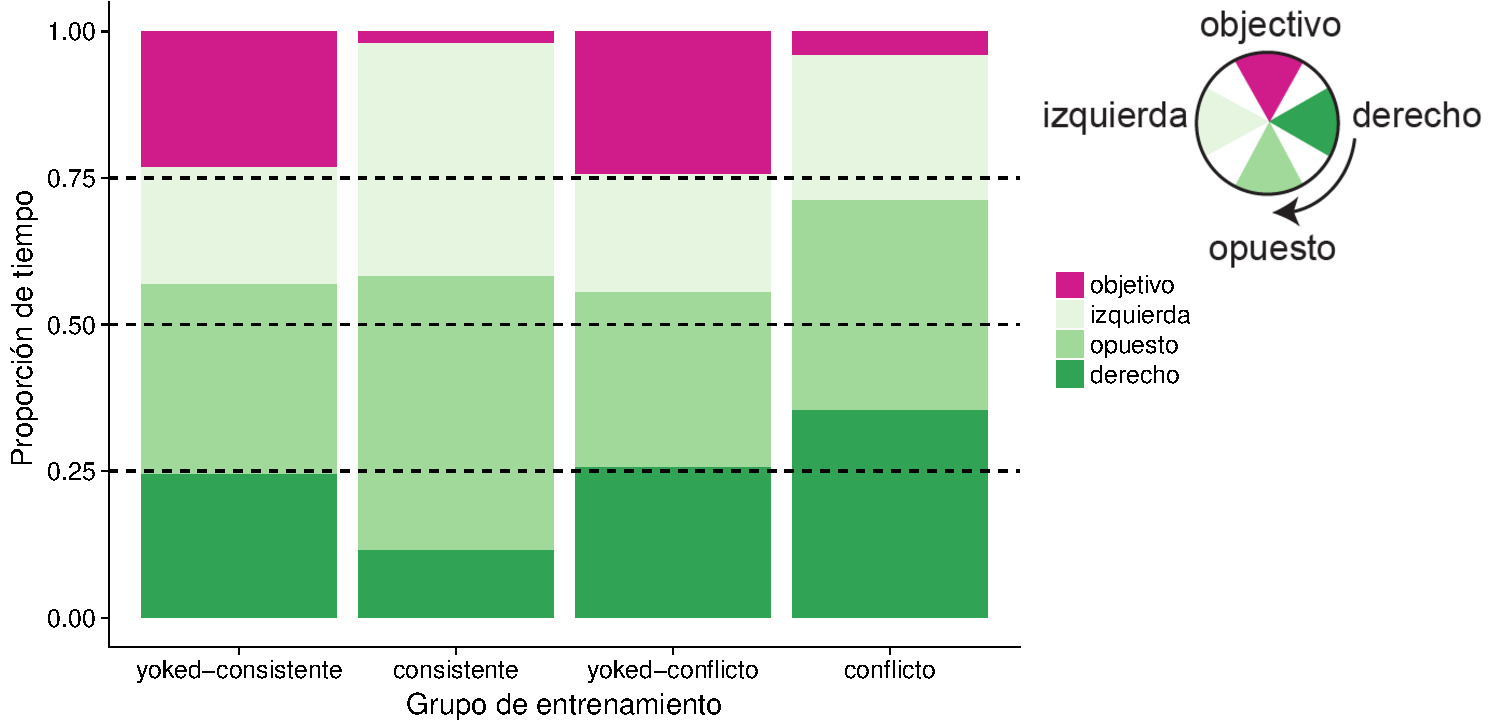
\includegraphics{../figures/10_talk/timespent2-1.pdf}

\begin{itemize}[<+->]
\tightlist
\item
  ``objetivo'', ``izquierda'', etc. son cuadrantes de una arena
\item
  Yo quería mostrar un uso desproporcionado del espacio
\item
  Use \textbf{cowplot}\footnote<.->{\textbf{cowplot}
    \url{https://cran.r-project.org/web/packages/cowplot/index.html}}
  para agregar imágenes dentro de R
\end{itemize}

\end{frame}

\begin{frame}{Deseo 3: Usa \emph{R Markdown} para la reproducibilidad}


\includegraphics[width=0.50000\textwidth]{../figures/10_talk/Rmarkdown.png}
\footnote<.->{\url{https://rmarkdown.rstudio.com/authoring_quick_tour.html}}

\end{frame}

\begin{frame}{Deseo 4: Usa el control de versiones para colaborar
con otros y con vos en el futuro}

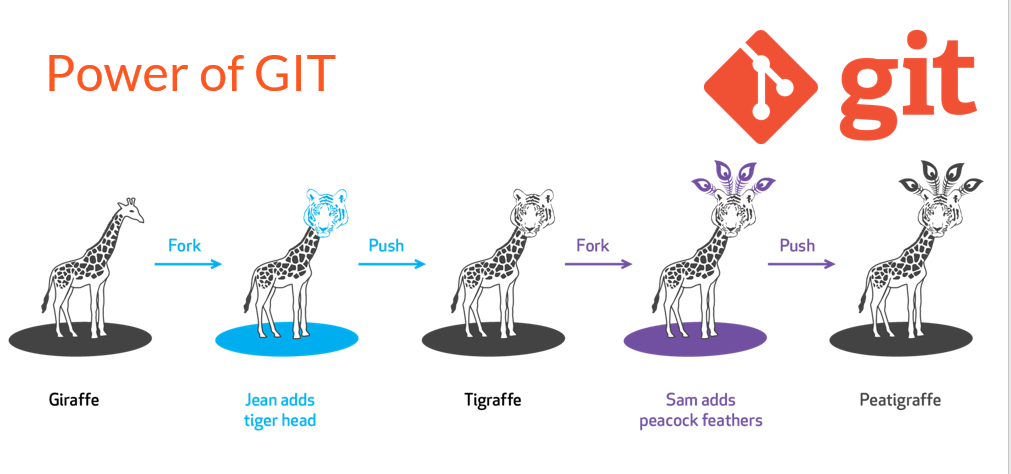
\includegraphics[width=0.75000\textwidth]{../figures/10_talk/git-graphic-01.png}
\footnote<.->{\url{http://technetnepal.net/blogs/shirishamaharjan/archive/2017/05/07/expand-horizons-change-attitudes-git-and-github-workshop.aspx}}

\end{frame}

\begin{frame}{Deseo 5: Documenta su flujo de trabajo}

Porque probablemente sea único y complejo

\includegraphics[width=0.75000\textwidth]{https://www.blogdelfotografo.com/wp-content/uploads/2016/05/mark-516279_1920.jpg}
\footnote<.->{\url{https://www.blogdelfotografo.com/workflow-flujo-trabajo-foto/}}

\end{frame}

\begin{frame}{Por ejemplo, puede enumerar los comandos por orden de
operación}

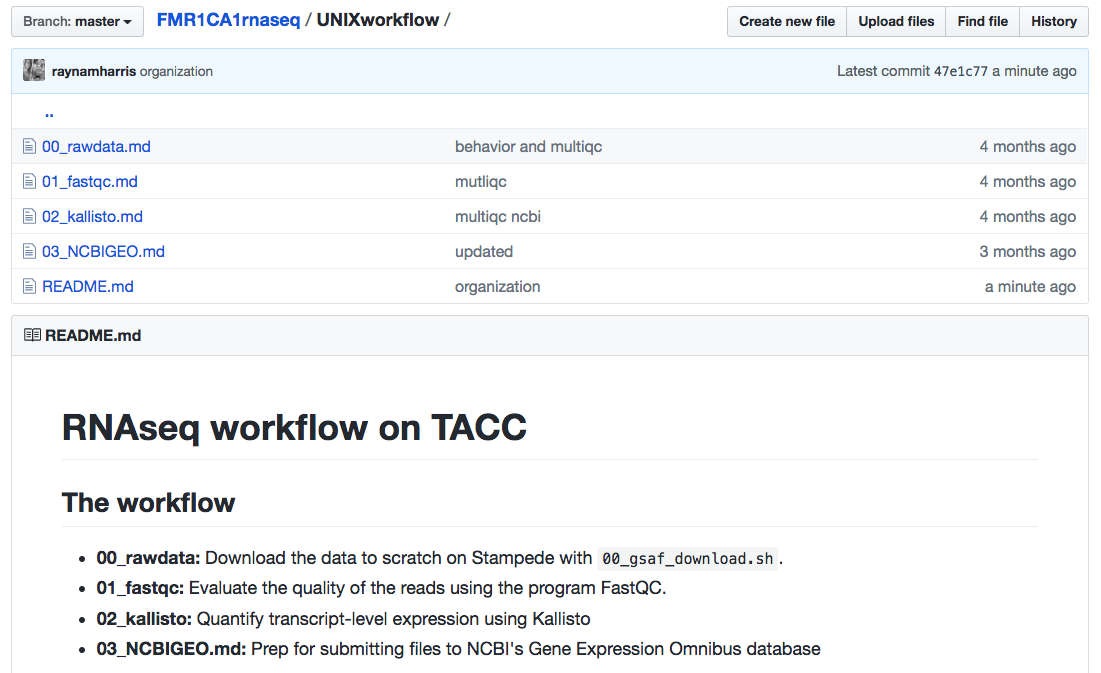
\includegraphics[width=0.75000\textwidth]{../figures/10_talk/unixworkflow.png}
\footnote<.->{\url{https://github.com/raynamharris/FMR1CA1rnaseq}}

\end{frame}

\begin{frame}{Pruebe múltiples estrategias de organización y haga lo que
funcione mejor para vos}

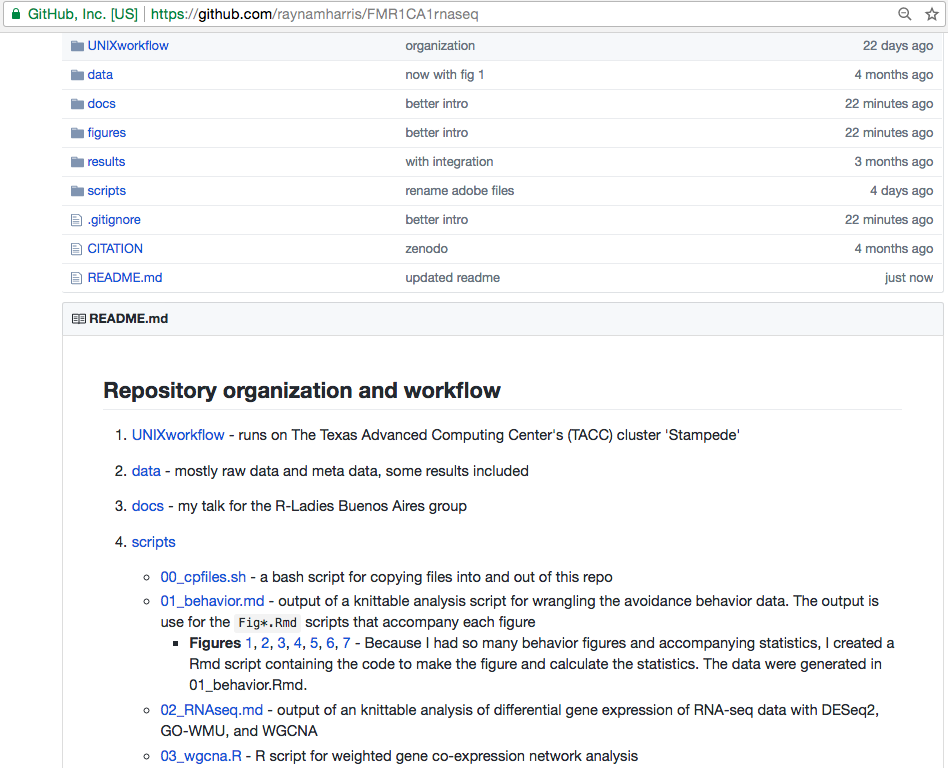
\includegraphics[width=0.75000\textwidth]{../figures/10_talk/Rworkflow.png}
\footnote<.->{\url{https://github.com/raynamharris/FMR1CA1rnaseq}}

\end{frame}

\begin{frame}{Punto medio resumen}

\begin{itemize}
\tightlist
\item
  Deseo 1: Desarrolla tu propia paleta de colores
\item
  Deseo 2: Usa leyendas graficas
\item
  Deseo 3: Usa \emph{R Markdown} para la reproducibilidad
\item
  Deseo 4: Usa el control de versiones para la colaboración
\item
  Deseo 5: Documenta su flujo de trabajo
\end{itemize}

\end{frame}

\begin{frame}{Deseo 6: Me ayuda mejor las nuevas lecciones en español de
Software Carpentry}

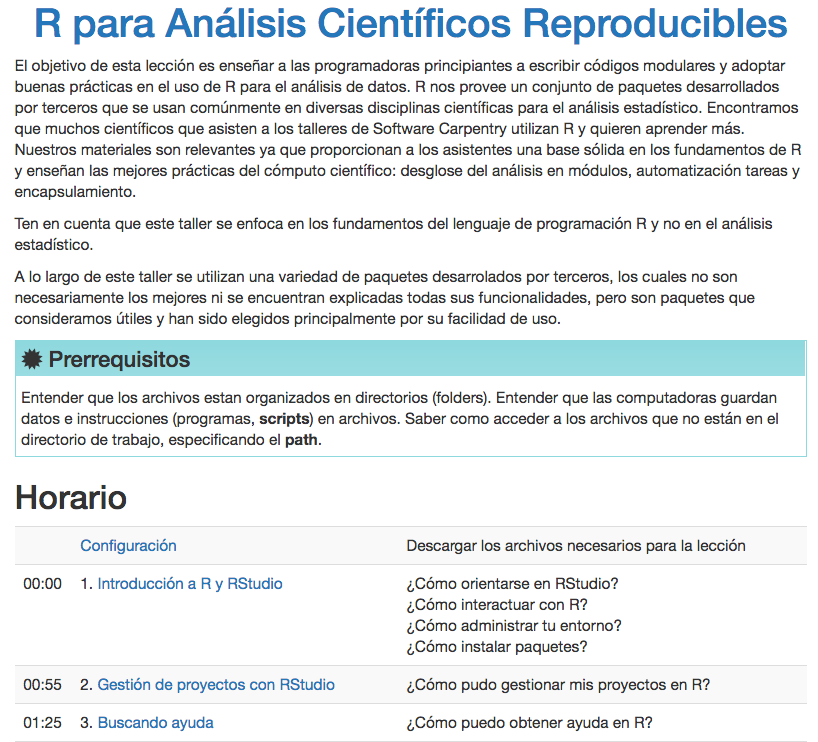
\includegraphics{../figures/10_talk/R-gapminder-es.png}

\end{frame}

\begin{frame}{Como podes ayudarme}

\begin{itemize}[<+->]
\tightlist
\item
  Leer y comentar o editar en GitHub\footnote<.->{\url{https://swcarpentry.github.io/r-novice-gapminder-es/}}
\item
  Particpar en el \textbf{Bug BBQ}\footnote<.->{\url{https://carpentries.github.io/2018-04-bug-bbq/}}
  el Abril 11 y 12
\item
  Haga videos de usted leyendo y codificando junto con la
  lección\footnote<.->{\url{https://www.youtube.com/watch?v=rQkfLaTdAvw}}
\end{itemize}

\end{frame}

\begin{frame}{Deseo 7: Convertirse en una instructor certificada}

\begin{itemize}
\tightlist
\item
  Ahora, no hay instructoras en Argentina :(
\item
  Aplica aquí: \url{http://carpentries.github.io/instructor-training/}
\end{itemize}

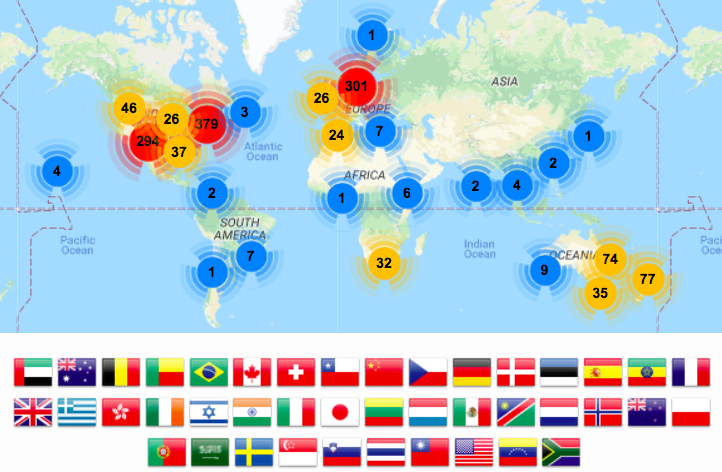
\includegraphics[width=0.75000\textwidth]{../figures/10_talk/joinus.png}
\footnote<.->{\url{https://software-carpentry.org/team/}}

\end{frame}

\begin{frame}{Deseo 8: Organizar y / o asistir a un taller}

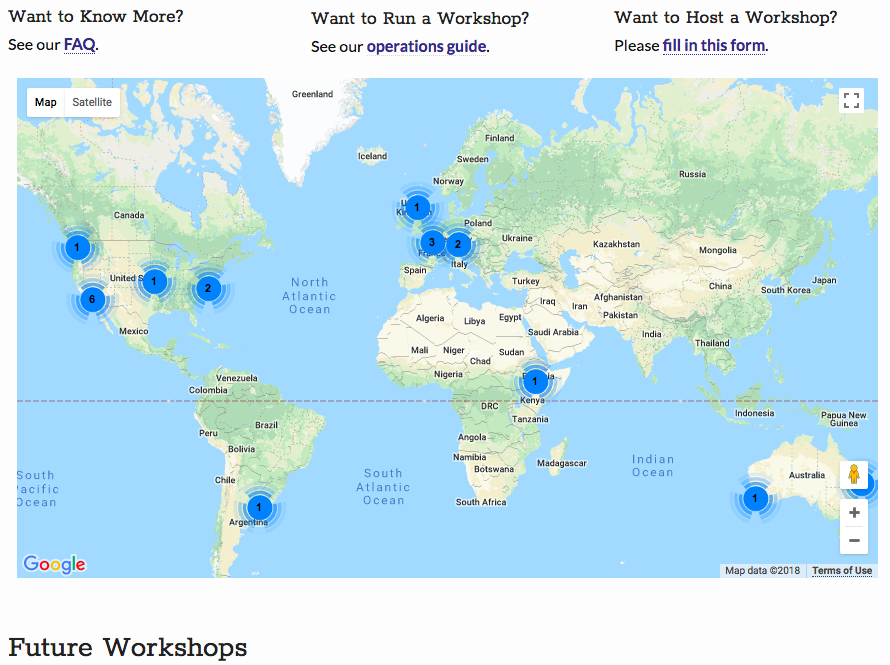
\includegraphics[width=0.75000\textwidth]{../figures/10_talk/workshops.png}
\footnote<.->{\url{https://software-carpentry.org/workshops/}}

\end{frame}

\begin{frame}{¡Gracias por tu atención! ¡Mantengamonos en contacto!}

Twitter: @raynamharris

Email:
\href{mailto:rayna.harris@gmail.com}{\nolinkurl{rayna.harris@gmail.com}}

\end{frame}

\end{document}
